% Task 2 report section for inclusion in the IEEE paper.
% Requires \usepackage{graphicx} in the main preamble.
% Copy the two selected PNG charts to report/ieee/figures/final_v1/.

\section{Experimental Evaluation}
\label{sec:task2-experiments}

\subsection{Experimental Setup}
The Tank Battle problem is modeled as a two-player, turn-based, zero-sum game. Four search configurations were evaluated: Minimax, Alpha-Beta, Heuristic Minimax, and Heuristic Minimax with Alpha-Beta pruning. Alpha-Beta eliminates branches that cannot change the Minimax decision value \cite{knuth1975analysis}. The baseline evaluator uses the difference between the current and opponent tank/base hit points (HP). The heuristic evaluator additionally considers reachable path distance to opponent assets, immediate movement mobility, and directional bullet threats. Its default weights are 12.0 for tank HP, 18.0 for base HP, 1.5 for distance, 1.0 for mobility, and 4.0 for bullet threat.

Four 13$\times$13 starting scenarios were used: (S1) the default map, (S2) an open map without walls, (S3) an obstacle map with a central passage, and (S4) a close-range combat map containing two active bullets. For each scenario, every algorithm received a fresh instance of the same initial state. Search depths were 2 and 3 plies, where one ply represents one player's action. Each scenario--algorithm--depth combination was measured 10 times, producing 320 measured runs. One unmeasured warm-up run was performed for each combination (32 warm-up runs in total). The algorithm execution order was shuffled using fixed seed 42 for reproducibility; the action ordering inside each search algorithm was not randomized.

The primary timing metric is wall-clock time for the complete \texttt{agent.search()} call, measured with Python's high-resolution performance counter. Process startup time is excluded. Node counts, evaluation scores, cutoffs, and pruned branches were also recorded. Pairwise validation confirmed that Minimax and Alpha-Beta returned matching evaluation scores under the baseline evaluator, and that the two heuristic configurations returned matching scores, for all tested scenario/depth/repetition groups.

The experiments were run on an ASUS ROG Strix G513IH laptop with an AMD Ryzen 7 4800H processor (8 physical cores, 16 logical processors), 7.42 GB of physical memory reported by Windows, Windows 11 (build 26300), and 64-bit Python 3.14.8. The assignment lists macOS 13.7.8 with an Intel Core i5 as its reference environment; therefore, the timings reported here represent the actual Windows/AMD test environment and should not be interpreted as macOS measurements.

\subsection{Results and Discussion}
Table~\ref{tab:task2-performance} reports the mean explored nodes and mean wall-clock time. Runtime values are averaged over the 10 repetitions in each scenario and then across the four scenarios.

\begin{table*}[!t]
\centering
\caption{Mean Search Cost Across the Four Scenarios}
\label{tab:task2-performance}
\scriptsize
\setlength{\tabcolsep}{7pt}
\begin{tabular}{lrrrr}
\hline
\textbf{Algorithm} & \textbf{Nodes ($d=2$)} & \textbf{Time (ms, $d=2$)} & \textbf{Nodes ($d=3$)} & \textbf{Time (ms, $d=3$)} \\
\hline
Minimax & 43.0 & 11.74 & 259.0 & 67.15 \\
Alpha-Beta & 18.0 & 5.10 & 59.0 & 15.60 \\
Heuristic Minimax & 43.0 & 49.47 & 259.0 & 292.35 \\
Heuristic Minimax + Alpha-Beta & 19.5 & 19.27 & 79.0 & 90.95 \\
\hline
\end{tabular}
\end{table*}

At depth 3, standard Alpha-Beta reduced the explored nodes from 259 to 59, a 77.22\% reduction compared with Minimax. Its mean runtime decreased from 67.15 ms to 15.60 ms, corresponding to a 4.30$\times$ speedup. At depth 2, the node count decreased from 43 to 18 (58.14\%), and the measured speedup was 2.30$\times$. These results show that pruning becomes increasingly valuable as the search depth grows, while the paired score validation indicates that pruning preserved the Minimax evaluation score for the tested cases.

The heuristic configuration has a higher evaluation cost because it performs additional path-distance, mobility, and bullet-threat calculations. At depth 3, Heuristic Minimax required 292.35 ms on average, compared with 67.15 ms for standard Minimax. Adding Alpha-Beta reduced the heuristic search from 259 to an average of 79 explored nodes (69.50\%) and improved runtime from 292.35 ms to 90.95 ms, a 3.21$\times$ speedup. However, the heuristic-plus-pruning configuration remained slower than standard Alpha-Beta. The corresponding depth-2 results show the same trade-off: heuristic pruning reduced the average node count from 43 to 19.5 and improved runtime by 2.57$\times$ relative to Heuristic Minimax.

\begin{table}[!t]
\centering
\caption{Alpha-Beta Improvement Relative to Its Minimax Baseline}
\label{tab:task2-pruning}
\scriptsize
\setlength{\tabcolsep}{3pt}
\begin{tabular}{lrrrr}
\hline
\textbf{Configuration} & \textbf{Node reduction} & \textbf{Node reduction} & \textbf{Speedup} & \textbf{Speedup} \\
 & \textbf{($d=2$)} & \textbf{($d=3$)} & \textbf{($d=2$)} & \textbf{($d=3$)} \\
\hline
Standard & 58.14\% & 77.22\% & 2.30$\times$ & 4.30$\times$ \\
Heuristic & 54.65\% & 69.50\% & 2.57$\times$ & 3.21$\times$ \\
\hline
\end{tabular}
\end{table}

The average node count for heuristic Alpha-Beta varies across maps (19.5 nodes at depth 2 and 79 nodes at depth 3), because the heuristic leaf scores affect where Alpha-Beta cutoffs occur. The open and combat scenarios generally required less time than the default and obstacle scenarios in the depth-3 measurements, although the size of the difference depends on the algorithm. This indicates that board structure and the initial tactical situation influence practical search cost.

The results have several limitations. Only four hand-crafted starting scenarios and two shallow search depths were tested; the experiment does not establish performance on all possible game states or prove stronger playing strength through match win rates. Runtime is hardware- and interpreter-dependent. The reported speedups should therefore be interpreted as measurements for the stated environment, while explored-node reductions provide a more implementation-independent indication of pruning effectiveness.

\begin{figure}[!t]
\centering
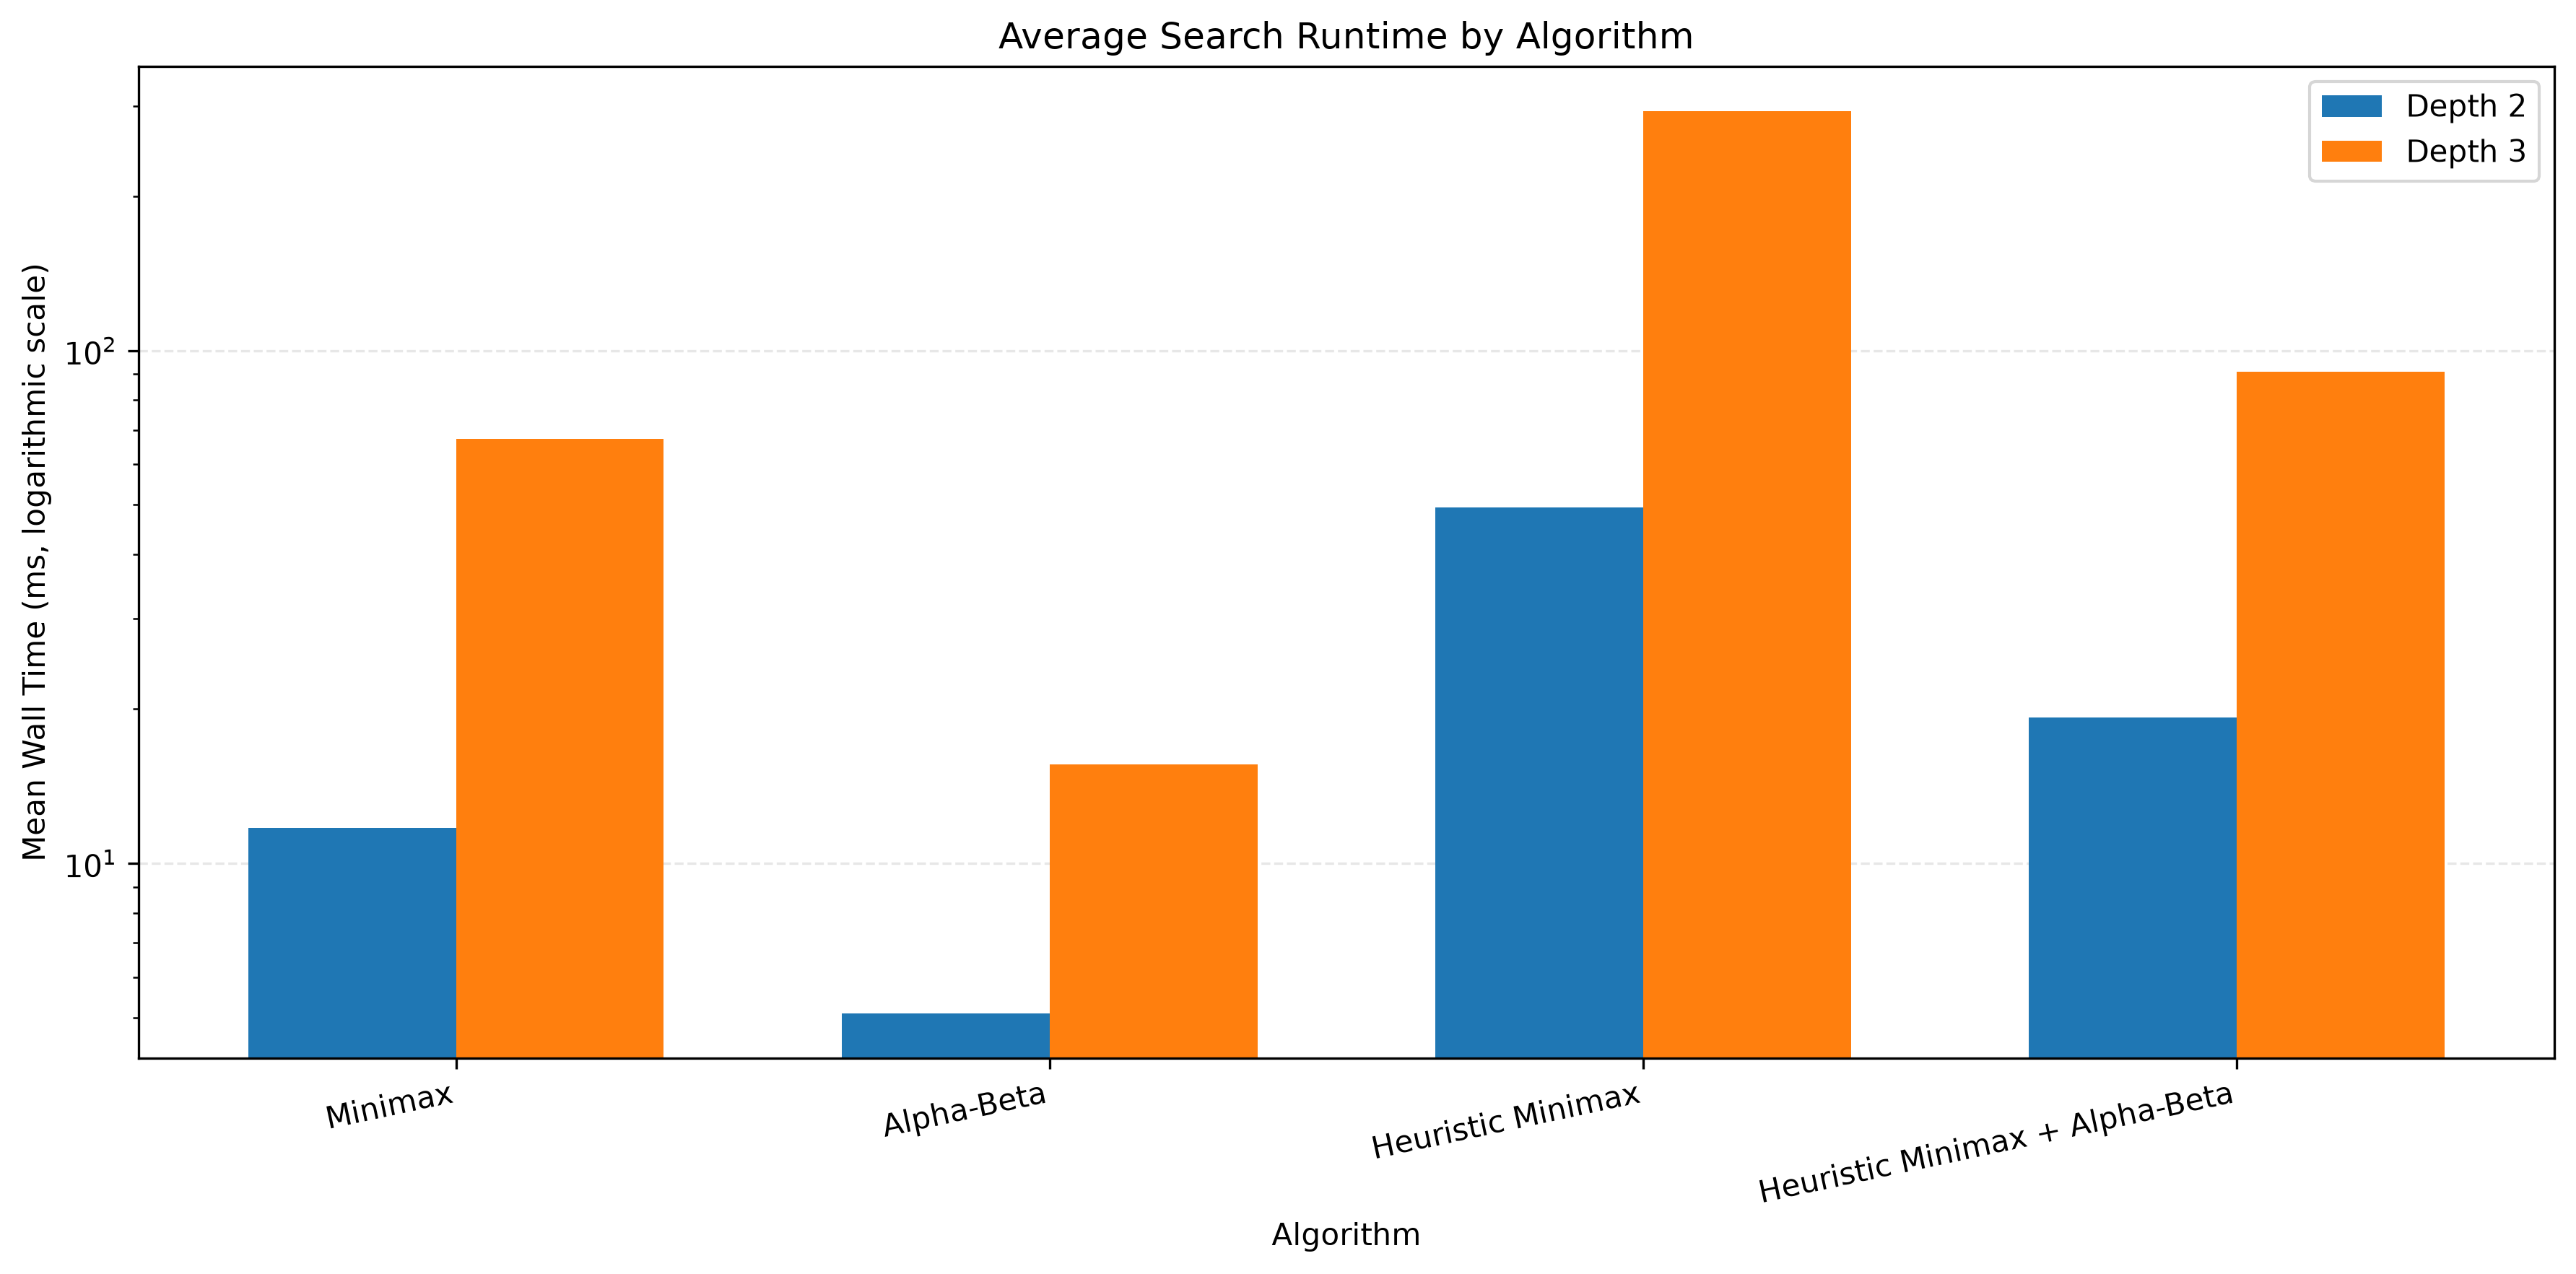
\includegraphics[width=\columnwidth]{figures/final_v1/mean_runtime_by_algorithm.png}
\caption{Mean wall-clock search time by algorithm and search depth.}
\label{fig:task2-runtime}
\end{figure}

\begin{figure}[!t]
\centering
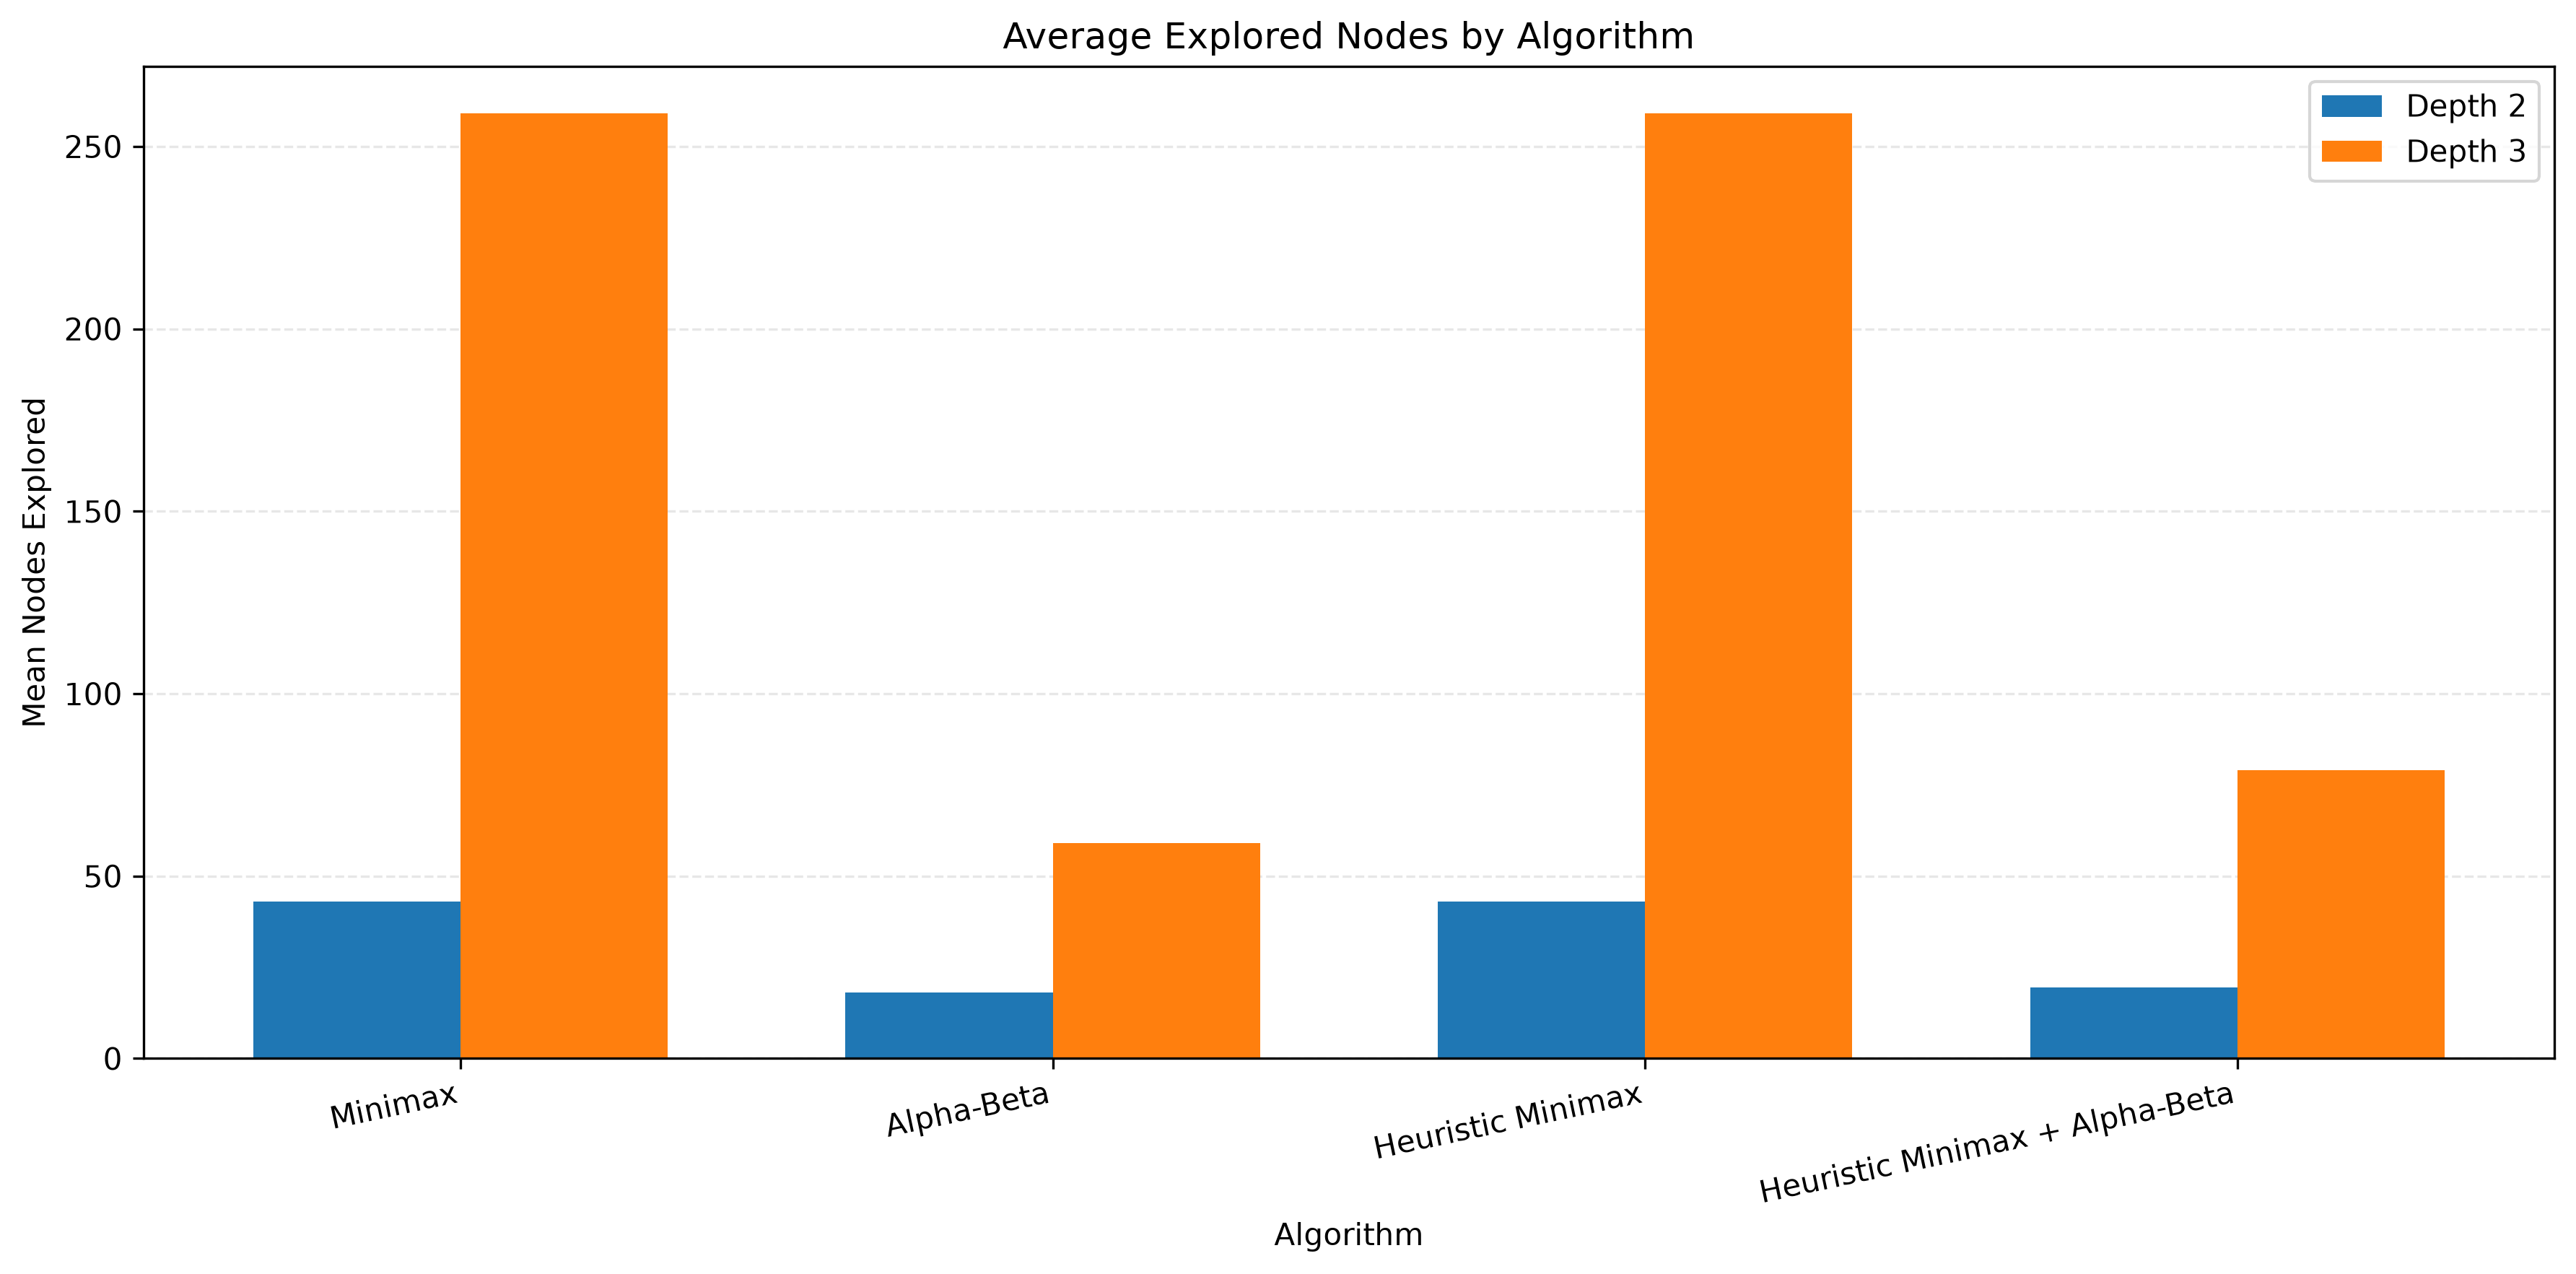
\includegraphics[width=\columnwidth]{figures/final_v1/mean_nodes_by_algorithm.png}
\caption{Mean number of explored nodes by algorithm and search depth.}
\label{fig:task2-nodes}
\end{figure}

\subsection{Conclusion}
The experiments demonstrate that Alpha-Beta pruning substantially reduces the search cost of both baseline and heuristic Minimax while preserving their paired evaluation scores in the tested cases. The largest reduction occurred at depth 3, where standard Alpha-Beta explored 77.22\% fewer nodes than Minimax. The heuristic evaluator provides richer state information but adds computational overhead; combining it with Alpha-Beta mitigates that cost, although it does not outperform standard Alpha-Beta in runtime. Overall, the results support using Alpha-Beta when computational efficiency is the priority and using the heuristic configuration when the additional strategic features justify its higher evaluation cost. Further evaluation with deeper searches, more diverse or randomized maps, and self-play win-rate measurements is left for future work.
